\documentclass{article}
\usepackage{amsmath}
\usepackage{amssymb}
\usepackage{tikz}
\usepackage{mathtools}
\usepackage{tkz-euclide}
\usepackage{pgf}
\usepackage{xcolor}
\usepackage{amsfonts}
\usepackage{graphicx}
\numberwithin{equation}{section}
\title{Fysikk}
\author{Martin N. Håvardsen}
\date{\today}
\begin{document}
\maketitle
\section{$K=\frac 1 2 mv^2$}
  \subsection{Grunnlag}
  Vi kan bruke $F=ma$ og $a=\frac{dv}{dt}=\frac{dv}{ds}\cdot\frac{ds}{dt}=\frac{dv}{ds}\cdot v$,
  \begin{align}
    F&=m\left(\frac{dv}{dt}\right) \\
    F&=m\cdot v\left(\frac{dv}{ds}\right)\\
    E=\int F\cdot ds&=\int m\cdot v\left(\frac{dv}{ds}\right) ds \\
    E&=m\cdot \int v\left(\frac{dv}{ds}\right)ds \\
    %\text{let $u$ be } &\text{a function where } \frac{du}{dv}\cdot\frac{dv}{ds}=\frac{du}{ds} \notag\\
    \text{let $u$ be } &\text{a function where } \frac{du}{dv}=v\notag\\
    E&=m\int\left(\frac{du}{dv}\right)\left(\frac{dv}{ds}\right)ds \\
    E&=m\int\left(\frac{du}{ds}\right)ds=m\left(u+C_1\right) \\
    E&=m\int vdv=m\left(\frac 1 2 v^2+C_2\right) \\
    E&=\frac 1 2 mv^2
  \end{align}
Merk at i likning \textbf{1.6} er $u=\displaystyle\int vdv$, og $C_1$ kan ignorerest. I likning \textbf{1.7} kan man ignorere $C_2$ siden $v=0\implies E=0$; $E$ har ingen konstantledd. 
\section{Energi fra miljøet}
  \begin{align}
    \Delta K= K_f-K_i=W \\
    \left.\Delta K= \text{}\right|
  \end{align}

\section{Distanse mellomg punkt og plan}\label{sec:Distanse mellomg punkt og plan} % (fold)

\begin{figure}[h]
\centering
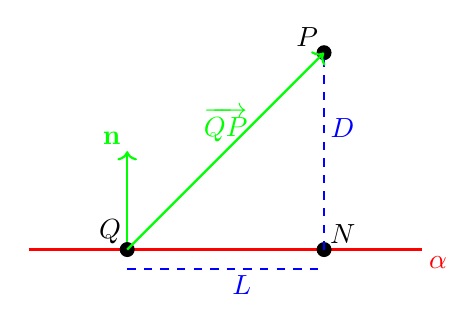
\begin{tikzpicture}[scale=2.5, every node/.style={inner sep=0pt}]
  % Left picture
  \begin{scope}[shift={(0,0)}]
    % grid
    %\draw[step=0.5cm,gray,very thin] (-0.5,-0.5) grid (1.5,1.5);
    % plane
    \draw[thick, red] (-0.5,0) -- (1.5,0.0) node [below right=0.1] {$\alpha$};
    % normal vector
    \draw[thick,->, green] (0,0) -- (0,0.5) node[above left=0.1] {$\bold{n}$};
    % points
    \filldraw[black] (0,0) circle (1pt) node [above left=0.1] {$Q$};
    \filldraw[black] (1,1) circle (1pt) node [above left=0.1] {$P$};
    \filldraw[black] (1,0) circle (1pt) node [above right=0.1] {$N$};
    % triangle edges
    \draw[thick, blue, dashed] (0,-0.1) -- (1.0,-0.1) node [pos=0.5, below right=0.1] {$L$};
    \draw[thick, blue, dashed] (1,0) -- (1.0,1.0) node [pos=0.7, below right=0.1] {$D$};
    \draw[thick, green, ->] (0,0) -- (1,1) node[pos=0.5, above=0.1] {$\overrightarrow{QP}$};
  \end{scope}
\end{tikzpicture}
  \caption{Plan og punkt}
\end{figure}

Vi har et plan git ved
\begin{equation}
  \alpha : \bold { n }\cdot(\overrightarrow{QX}) = 0
  \label{eq:alfa plan}
\end{equation}
der $Q$ er et punkt i planet $\alpha$ og $\bold {n}$, normalvektoren til planet. $P$ er et punkt  med distanse $D$ fra planet $\alpha$. 
Lengden $L$ er lengden langs plan $\alpha$ til punktet $N=P_{proj}$ der $\overrightarrow{PP_{proj}} \parallel \bold n$. La $\bold{v}=\overrightarrow{QP}\times\overrightarrow{NP}$
\begin{equation}
  L\triangleq\frac{|\overrightarrow{QP}\times\overrightarrow{NP}|}{|\overrightarrow{QP}|}
  \label{eq:L}
\end{equation}
Siden $\overrightarrow{QP}\perp\overrightarrow{QP_{proj}}$ har vi at
\begin{equation}
  D^2+L^2=|\overrightarrow{QP}|^2
  \label{eq:D 1}
\end{equation}
med substitusjon
\begin{equation}
  D=\displaystyle\frac{\sqrt{|\overrightarrow{QP}|^2 - |\overrightarrow{QP}\times\overrightarrow{NP}|^2}}{|\overrightarrow{QP}|}
  \label{eq:D 2}
\end{equation}

\begin{equation}
  D=\displaystyle\frac{\sqrt{|\overrightarrow{QP}|^2 - |\overrightarrow{QP}\times\overrightarrow{NP}|^2}}{|\overrightarrow{QP}|}
  \label{eq:exapnded D 1}
\end{equation}

\begin{align}
  \bold{v} = \overrightarrow{QP}\times\overrightarrow{NP}
  &=
  \det\begin{bmatrix}
    \bold{j} & \bold{i} & \bold{k} \\
    &\overrightarrow{QP}^T&\\
    &\overrightarrow{NP}^T&\\
  \end{bmatrix}
  \\
  &=
  \det\begin{bmatrix}
    \bold{j} & \bold{i} & \bold{k} \\
    QP_x&QP_y&QP_z\\
    NP_x&NP_y&NP_z\\
  \end{bmatrix}
  \\
  &=
    \bold{j}(QP_{y} \; QN_{z} - QP_{z} \; QN_{y})\\
    &\quad+\bold{i}(QP_{z} \; QN_{x} - QP_{x} \; QN_{z})\\
    &\quad+\bold{k}(QP_{x} \; QN_{y} - QP_{y} \; QN_{x}) 
  \\
  &=
  \begin{bmatrix}
    QP_{y} \; QN_{z} - QP_{z} \; QN_{y}\\
    QP_{z} \; QN_{x} - QP_{x} \; QN_{z}\\
    QP_{x} \; QN_{y} - QP_{y} \; QN_{x} 
  \end{bmatrix}
  \label{eq:crossprod}
\end{align}

Vi finner magnituden til $\bold {v} = \overrightarrow{QP}\times\overrightarrow{NP}$
\begin{align}
  |\overrightarrow{QP}\times\overrightarrow{NP}|^2&=
    \quad(QP_{y} \; QN_{z} - QP_{z} \; QN_{y})^2\\
    &\quad +(QP_{z} \; QN_{x} - QP_{x} \; QN_{z})^2\\
    &\quad +(QP_{x} \; QN_{y} - QP_{y} \; QN_{x})^2\\
    &= 
    v_x^2+v_y^2+v_z^2
\end{align}
Vi finner magnituden til $\overrightarrow{QP}$
\begin{align}
  |\overrightarrow{QP}|^2=
    QP_{x}^2
    +QP_{y}^2
    +QP_{z}^2
\end{align}

med substitusjon

\begin{equation}
  D=\displaystyle\sqrt{\frac
  {
    QP_{x}^2
    +QP_{y}^2
    +QP_{z}^2
  - (
  v_x^2+v_y^2+v_z^2
  )
  }
  {
    QP_{x}^2
    +QP_{y}^2
    +QP_{z}^2
  }
  }
  \label{eq:D 3}
\end{equation}

Vi tar føre oss skalarproduktet mellom $\overrightarrow{QP}$ og $\bold{n}$
\begin{align}
  |\overrightarrow{QP}\cdot\bold{n}|&=\Big{|}\;|\overrightarrow{QP}|\;|\bold{n}|\cos{\theta}\;\Big{|} \\
  &=|\overrightarrow{QP}|\;|\bold{n}|\;\big|\sin\left({\theta+\frac{\pi}{2}}\right)\big|
\end{align}
% section Distanse mellomg punkt og plan (end)

\end{document}
